\documentclass[a4paper,10pt]{article}
\usepackage{amssymb, amsmath, amsbsy, amsfonts}    % ECUACIONES Y SÍMBOLOS MATEMÁTICOS
\usepackage[utf8]{inputenc}              % CODIFICACIÓN UTF8, PARA Ñs Y ACENTOS Y DEMÁS
\usepackage{graphicx}
\usepackage[letterpaper, top=1cm, bottom=1.8cm,right=1.5cm,left=1.5cm]{geometry}
\usepackage{subfigure}
\usepackage{verbatim}




\begin{document}

\section{Conjunto de datos}
\begin{enumerate}
 \item \textbf{BAO}: BAO-BOSS-DR12, 6 puntos\footnote{revisar el archivo \texttt{montepython3-1/data/BAO$\_$consensus$\_$results$\_$dM$\_$Hz.txt}}\\
   - Nombre del likelihood: \texttt{bao$\_$boss$\_$dr12}
 
 \vspace{.2cm}
 \begin{tabular}{c|c|c}
 \hline
  z & distance-type & value \\ \hline
  0.38 & dM(rsfid/rs) & 1512.39 \\
  0.38 & Hz(rs/rsfid) & 81.2087 \\
  0.51 & dM(rsfid/rs) & 1975.22 \\
  0.51 & Hz(rs/rsfid) & 90.9029 \\
  0.61 & dM(rsfid/rs) & 2306.68 \\
  0.61 & Hz(rs/rsfid) & 98.9647 \\
 \hline
 \end{tabular}
 
 \item \textbf{Supernovas}: SDSS-II Joint Light-curve Analysis (JLA), 740 puntos\footnote{revisar el archivo \texttt{montepython3-1/data/JLA/jla$\_$lcparams.txt}}\\
   - Nombre del likelihood: \texttt{JLA}\\
   - Se fijaron los valores de los \textit{nuisance parameters} de acuerdo con [arXiv:1401.4064v2, tabla 15, fila 1] 
   
   \begin{itemize}
    \item $\alpha$ = 0.141
    \item $\beta$ = 3.099
    \item M = -19.09
    \item $\Delta$M = -0.070
   \end{itemize}

 \item \textbf{CMB}: Planck TT + lowP (2015), [NUMERO DE DATOS?] \\
   - Nombre de los likelihoods: \texttt{Planck$\_$highl, Planck$\_$lowl} \\
   - low-$\ell$ = $\{\ell=2, \ell=29\}$, high-$\ell$ = $\{\ell=30, \ell=2508\}$ \\
   - Se fijaron los valores de los \textit{nuisance parameters} de acuerdo con el archivo de montepython \texttt{base2015.param}
   
\begin{figure}[h]
 \centering
 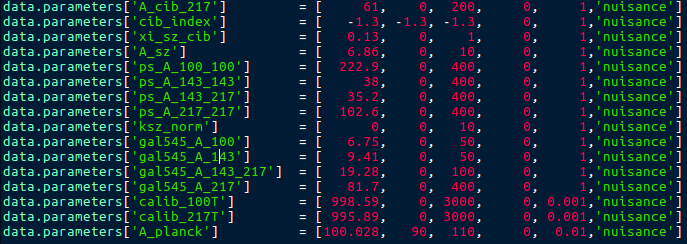
\includegraphics[scale=0.6]{planck_nuisance_parameters.png}
 \caption{\footnotesize{[mean, min, max, 1-sigma, scale, 'role']}}
\end{figure}


\end{enumerate}

\begin{comment}
\begin{figure}[h]
 \centering
 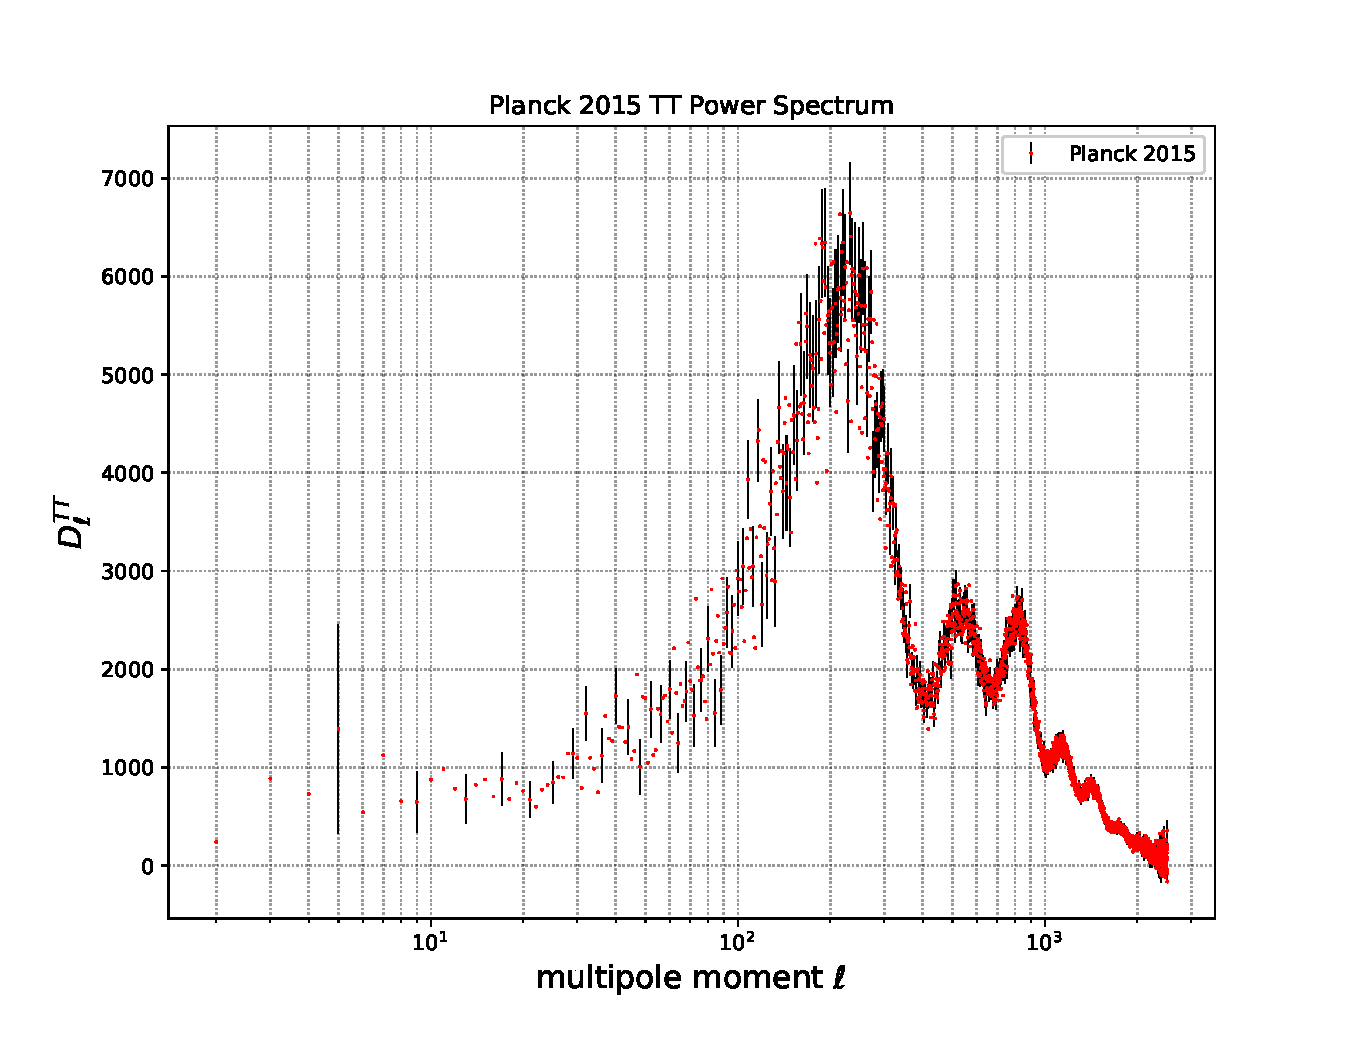
\includegraphics[scale=0.6]{planck_2015_Dl.pdf}
 %\caption{\footnotesize{[mean, min, max, 1-sigma, scale, 'role']}}
\end{figure}
\end{comment}

\section{Comparación de dos parametrizaciones 2-dim $(a,b)$ equivalentes} %(CPL y w(N=1) con BAO+JLA }
\subsection{CPL}

\begin{tabular}{|l|c|c|c|c|c|c|} 
 \hline 
 & & & \multicolumn{4}{ |c| }{Marginal Limits} \\  
 Param & best-fit & mean $\pm \sigma$ & \multicolumn{2}{ |c| }{68\%} & \multicolumn{2}{ |c| }{95\%}   \\ 
 & & & lower & upper  & lower & upper \\ \hline 
 $100~\omega_{b }$ &$1.625$ & $1.196_{-0.7}^{+0.12}$ & $0.50$ & $1.3120$ & $0.5$ & $2.551$ \\ 
 $\omega_{cdm }$ &$0.1488$ & $0.1751_{-0.019}^{+0.04}$ & $0.15583$ & $0.21553$ & $0.1021$ & $0.2301$ \\ \hline
 $w0_{fld }$ &$-1.102$ & $-1.011_{-0.22}^{+0.22}$ & $-1.229$ & $-7.91$ & $-1.441$ & $-0.5831$ \\ 
 $wa_{fld }$ &$-0.1441$ & $-2.133_{-0.52}^{+2}$ & $-0.26492$ & $-0.1$ & $-5.487$ & $-0.1$ \\ \hline
 $\Omega_{\Lambda }$ &$0.6483$ & $0.5989_{-0.071}^{+0.041}$ & $0.12593$ & $0.52793$ & $0.4944$ & $0.7248$ \\ 
 $H0$ &$68.5$ & $68.29_{-0.82}^{+0.81}$ & $67.46$ & $69.10$ & $66.67$ & $69.93$ \\ 
 \hline 
 \end{tabular}
 
\medskip
$-\ln{\cal L}_\mathrm{min} =343.001$, minimum $\chi^2=686$ 

\vspace{.5cm}
\subsection{w(N=1)}

\vspace{.2cm}
\begin{tabular}{|l|c|c|c|c|c|c|} 
 \hline 
 & & & \multicolumn{4}{ |c| }{Marginal Limits} \\  
 Param & best-fit & mean $\pm \sigma$ & \multicolumn{2}{ |c| }{68\%} & \multicolumn{2}{ |c| }{95\%}   \\ 
 & & & lower & upper  & lower & upper \\ \hline 
 $100~\omega_{b }$ &$2.589$ & $1.426_{-0.93}^{+0.2}$ & $0.5$ & $1.6226$  & $0.5$ & $3.093$ \\ 
 $\omega_{cdm }$ &$0.1063$ & $0.1638_{-0.024}^{+0.05}$ & $0.13981$ & $0.21387$ & $0.0823$ & $0.2273$ \\ \hline 
 $b0_{fld }$ &$-1.042$ & $-1.055_{-0.22}^{+0.24}$ & $-1.2717$ & $-0.81614$ & $-1.515$ & $-0.6057$ \\  
 $b1_{fld }$ &$-0.2704$ & $-2.418_{-0.61}^{+2.3}$ & $-3.0262$ & $-0.1$ & $-5.878$ & $-0.1$ \\ \hline
 $\Omega_{\Lambda }$ &$0.7194$ & $0.6196_{-0.085}^{+0.05}$ & $0.53413$ & $0.66982$ & $0.5039$ & $0.759$ \\ 
 $H0$ &$68.65$ & $68.42_{-0.84}^{+0.83}$ & $67.587$ & $69.256$ & $66.76$ & $70.1$ \\ 
 \hline 
 \end{tabular}
 
\medskip 
$-\ln{\cal L}_\mathrm{min} =342.922$, minimum $\chi^2=685.8$ 

\begin{figure}[t]
 \centering     %%% not \center
 \subfigure[CPL]{\label{fig:S3_1}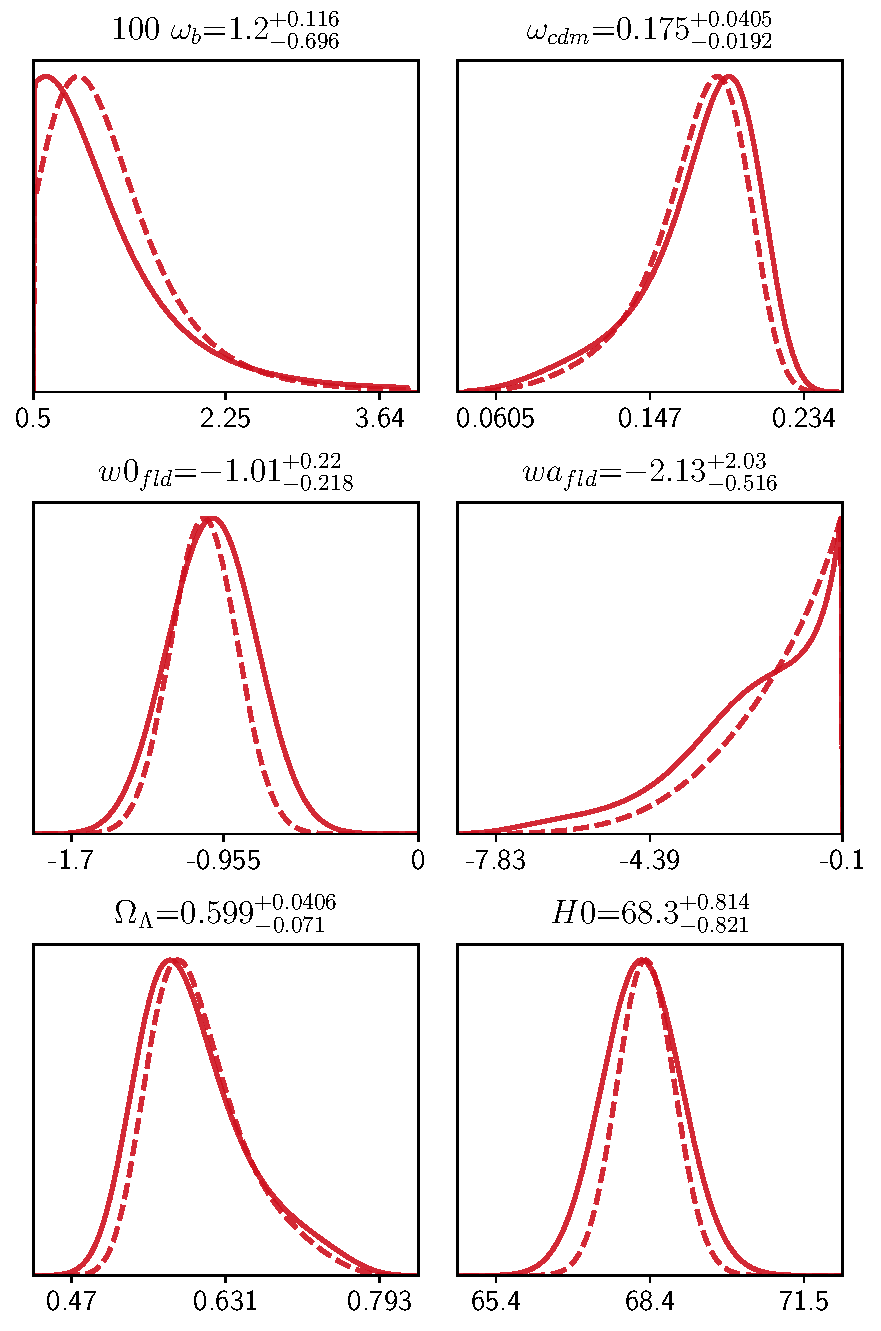
\includegraphics[scale=0.55]{cpl_19-4-1_1d.pdf}}
 \subfigure[w(N=1)]{\label{fig:S3_2}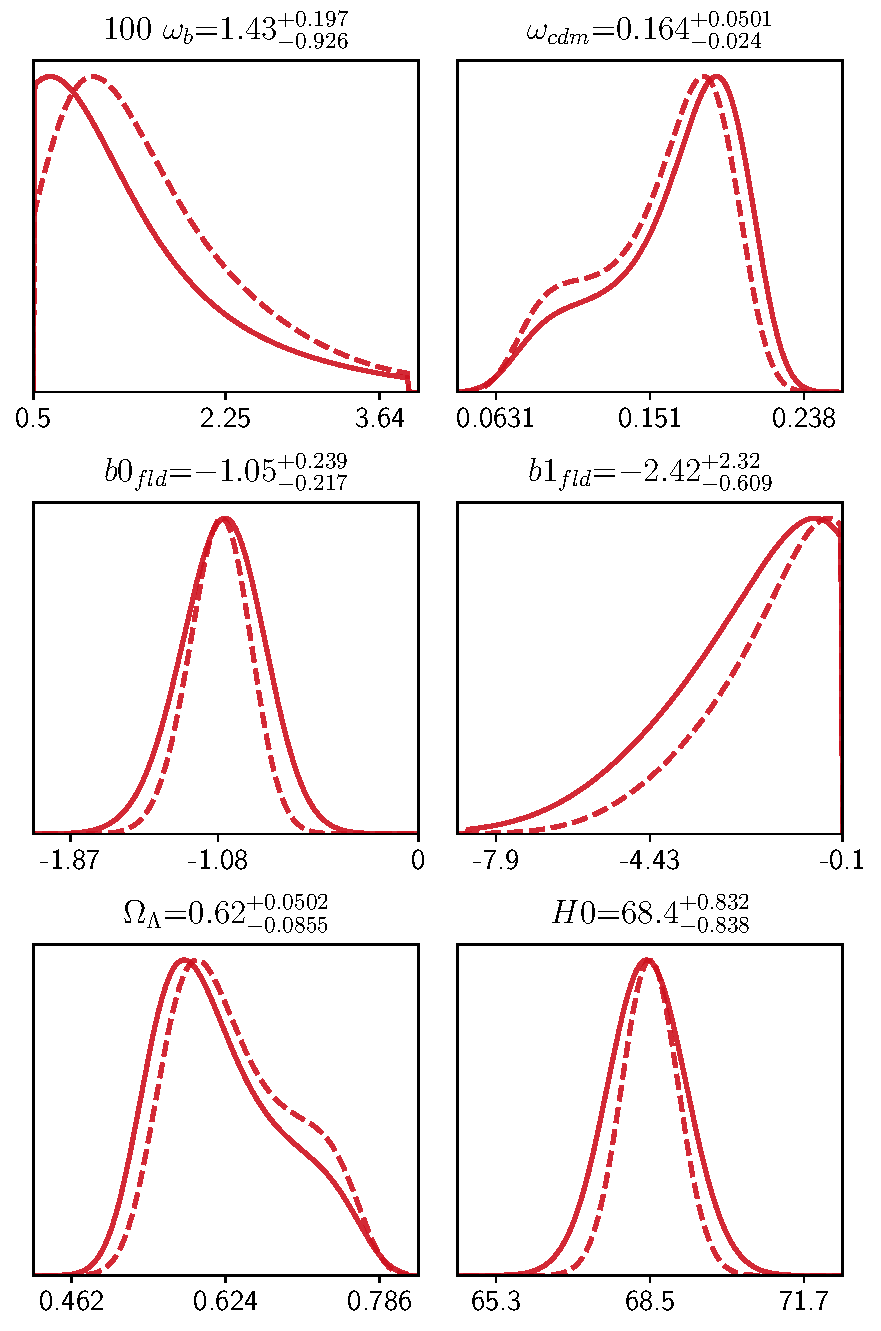
\includegraphics[scale=0.55]{nrk_19-3-1_f1-7_1d.pdf}}
 %\caption{\footnotesize{Un 3-espacio con curvatura positiva constante es la 3-esfera, a este universo se le llama \textbf{cerrado} y tiene la peculiaridad de contener líneas de mundo cerradas.
% Se muestra aquí una 2-esfera $S^2$ como referencia}}
\end{figure}

\begin{comment}

\begin{figure}[h]
 \centering
 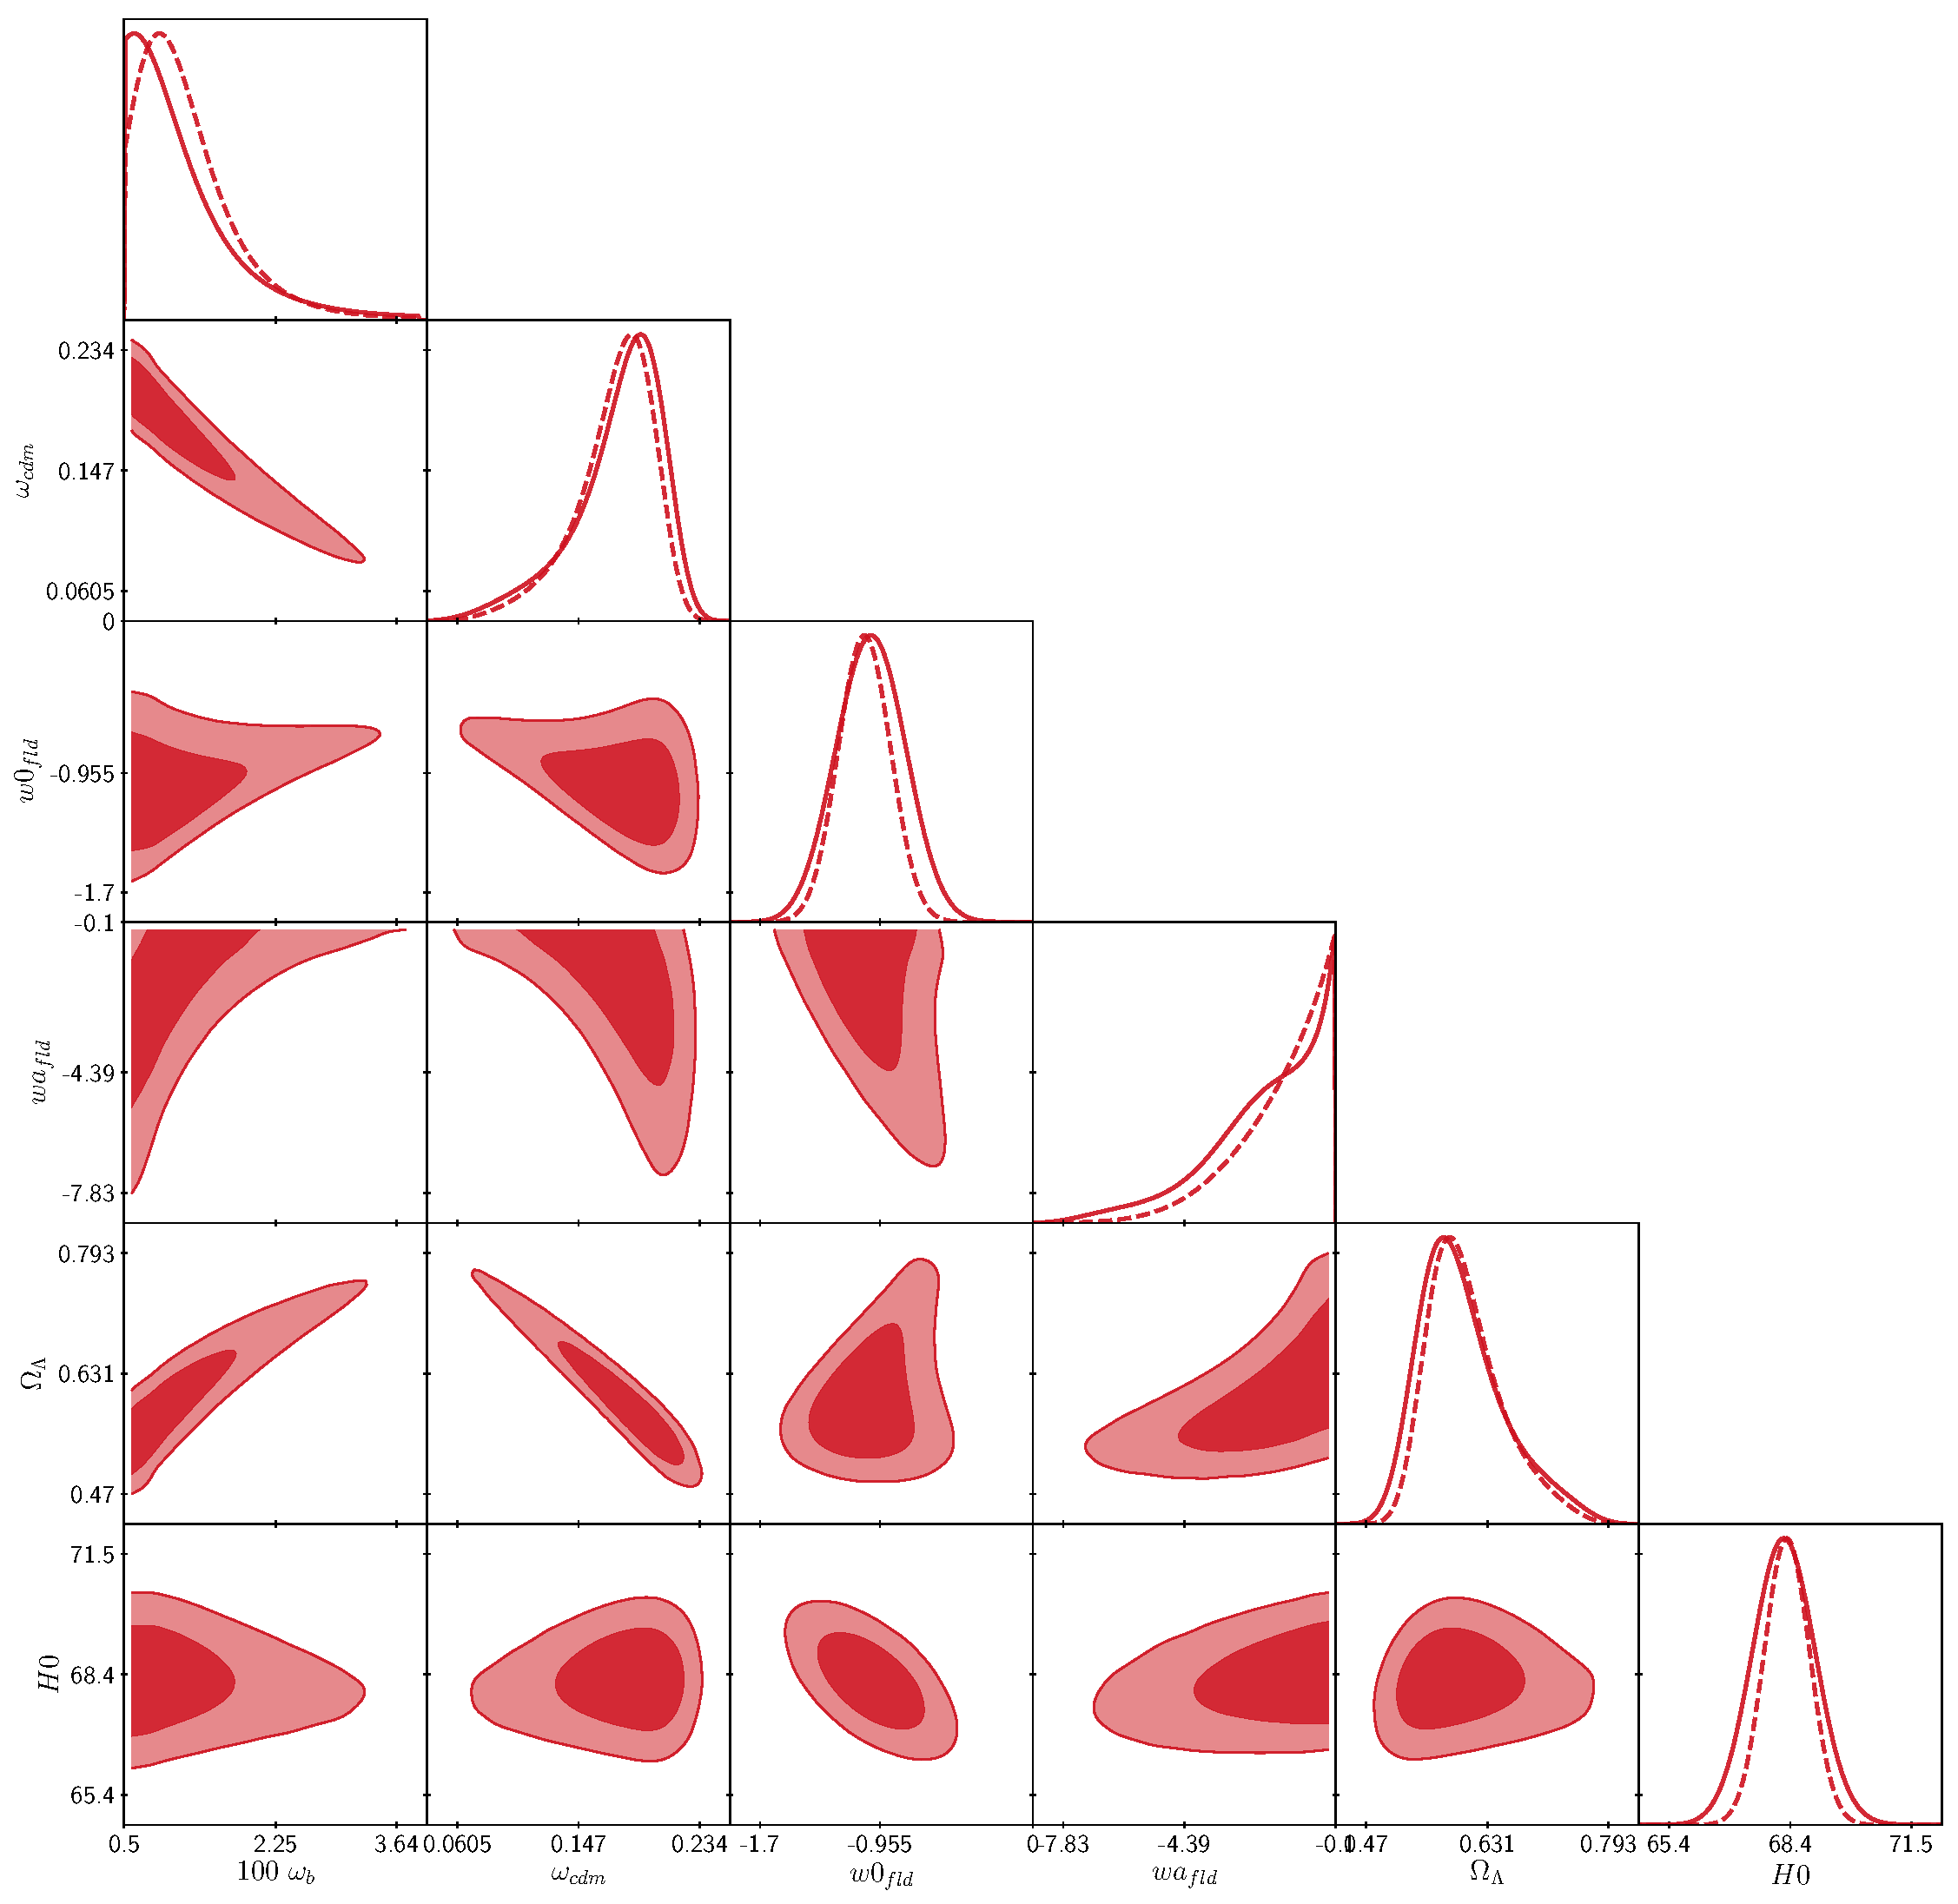
\includegraphics[scale=0.6]{cpl_19-4-1_triangle.pdf}
 %\caption{\footnotesize{[mean, min, max, 1-sigma, scale, 'role']}}
\end{figure}
\begin{figure}[h]
 \centering
 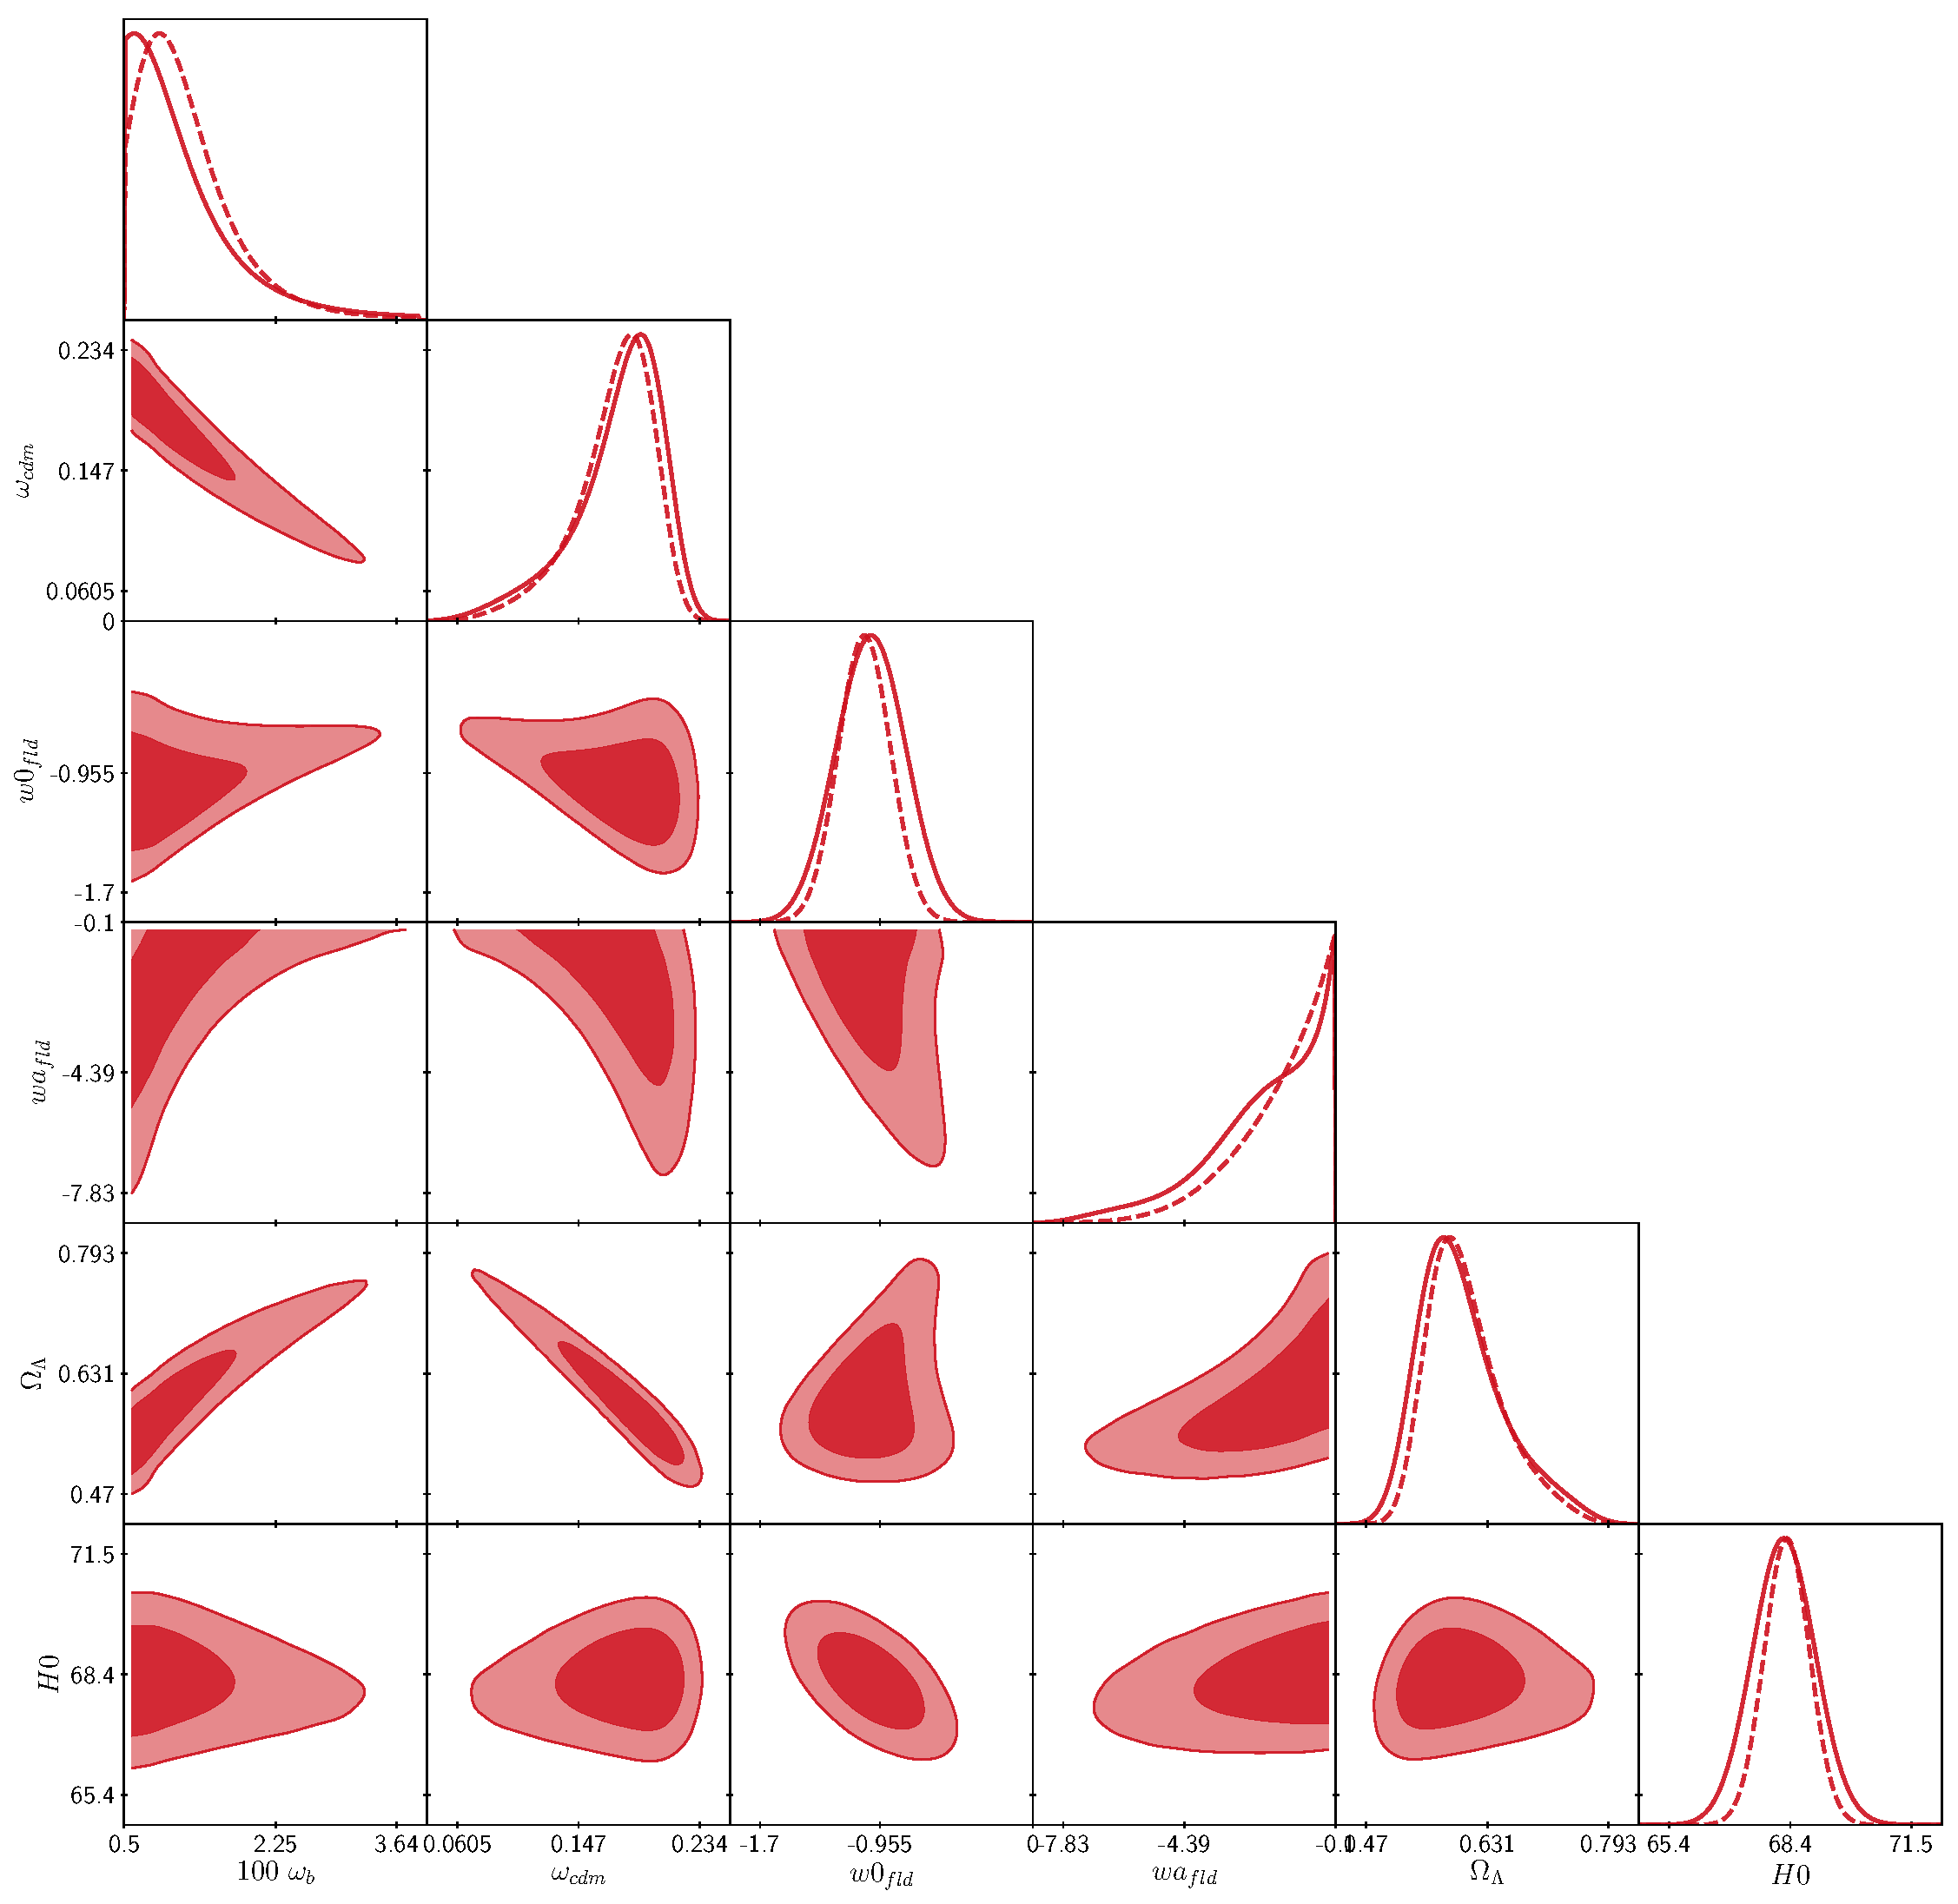
\includegraphics[scale=0.3]{cpl_19-4-1_triangle.pdf}
 %\caption{\footnotesize{[mean, min, max, 1-sigma, scale, 'role']}}
\end{figure}
\end{comment}

\section{Resultados BAO+JLA vs Planck+BAO+JLA}
\subsection{w(N=1)}

\begin{itemize}
 \item BAO+JLA, 1.2m de pasos, 8 procesos, convergencia de todos los parámetros
 \item Planck+BAO+JLA, 950k pasos, 8 procesos, convergencia de todos los parámetros
\end{itemize}

\begin{tabular}{|l|c|c|c|c|} 
 \hline 
Param & best-fit & mean$\pm\sigma$ & 95\% lower & 95\% upper \\ \hline 
$100~\omega_{b }$ &$2.589$ & $1.426_{-0.93}^{+0.2}$ & $0.5$ & $3.093$ \\ 
$\omega_{cdm }$ &$0.1063$ & $0.1638_{-0.024}^{+0.05}$ & $0.0823$ & $0.2273$ \\ 
$b0_{fld }$ &$-1.042$ & $-1.055_{-0.22}^{+0.24}$ & $-1.515$ & $-0.6057$ \\ 
$b1_{fld }$ &$-0.2704$ & $-2.418_{-0.61}^{+2.3}$ & $-5.878$ & $-0.1$ \\ 
$\Omega_{\Lambda }$ &$0.7194$ & $0.6196_{-0.085}^{+0.05}$ & $0.5039$ & $0.759$ \\ 
$H0$ &$68.65$ & $68.42_{-0.84}^{+0.83}$ & $66.76$ & $70.1$ \\ 
\hline 
 \end{tabular} \\ 
$-\ln{\cal L}_\mathrm{min} =342.922$, minimum $\chi^2=685.8$ \\ 

\begin{tabular}{|l|c|c|c|c|} 
 \hline 
Param & best-fit & mean$\pm\sigma$ & 95\% lower & 95\% upper \\ \hline 
$100~\omega_{b }$ &$2.238$ & $2.238_{-0.018}^{+0.018}$ & $2.202$ & $2.275$ \\ 
$\omega_{cdm }$ &$0.1191$ & $0.1192_{-0.0019}^{+0.0019}$ & $0.1155$ & $0.1231$ \\ 
$10^{+9}A_{s }$ &$2.264$ & $2.245_{-0.079}^{+0.075}$ & $2.091$ & $2.401$ \\ 
$n_{s }$ &$0.9697$ & $0.9699_{-0.0049}^{+0.0048}$ & $0.9603$ & $0.9795$ \\ 
$\tau_{reio }$ &$0.09225$ & $0.08777_{-0.018}^{+0.018}$ & $0.05146$ & $0.1236$ \\ 
$b0_{fld }$ &$-0.9266$ & $-0.9242_{-0.13}^{+0.12}$ & $-1.17$ & $-0.6762$ \\ 
$b1_{fld }$ &$-1.28$ & $-1.331_{-0.29}^{+0.39}$ & $-2.05$ & $-0.6609$ \\ 
$\Omega_{\Lambda }$ &$0.6961$ & $0.6968_{-0.0079}^{+0.0083}$ & $0.6805$ & $0.7129$ \\ 
$z_{reio }$ &$11.19$ & $10.75_{-1.5}^{+1.7}$ & $7.565$ & $13.87$ \\ 
$H0$ &$68.24$ & $68.35_{-0.79}^{+0.77}$ & $66.81$ & $69.93$ \\ 
$\sigma8$ &$0.8471$ & $0.8453_{-0.019}^{+0.019}$ & $0.808$ & $0.8823$ \\ 
\hline 
 \end{tabular} \\ 
$-\ln{\cal L}_\mathrm{min} =5987.82$, minimum $\chi^2=1.198e+04$ \\ 


\begin{figure}[h]
 \centering
 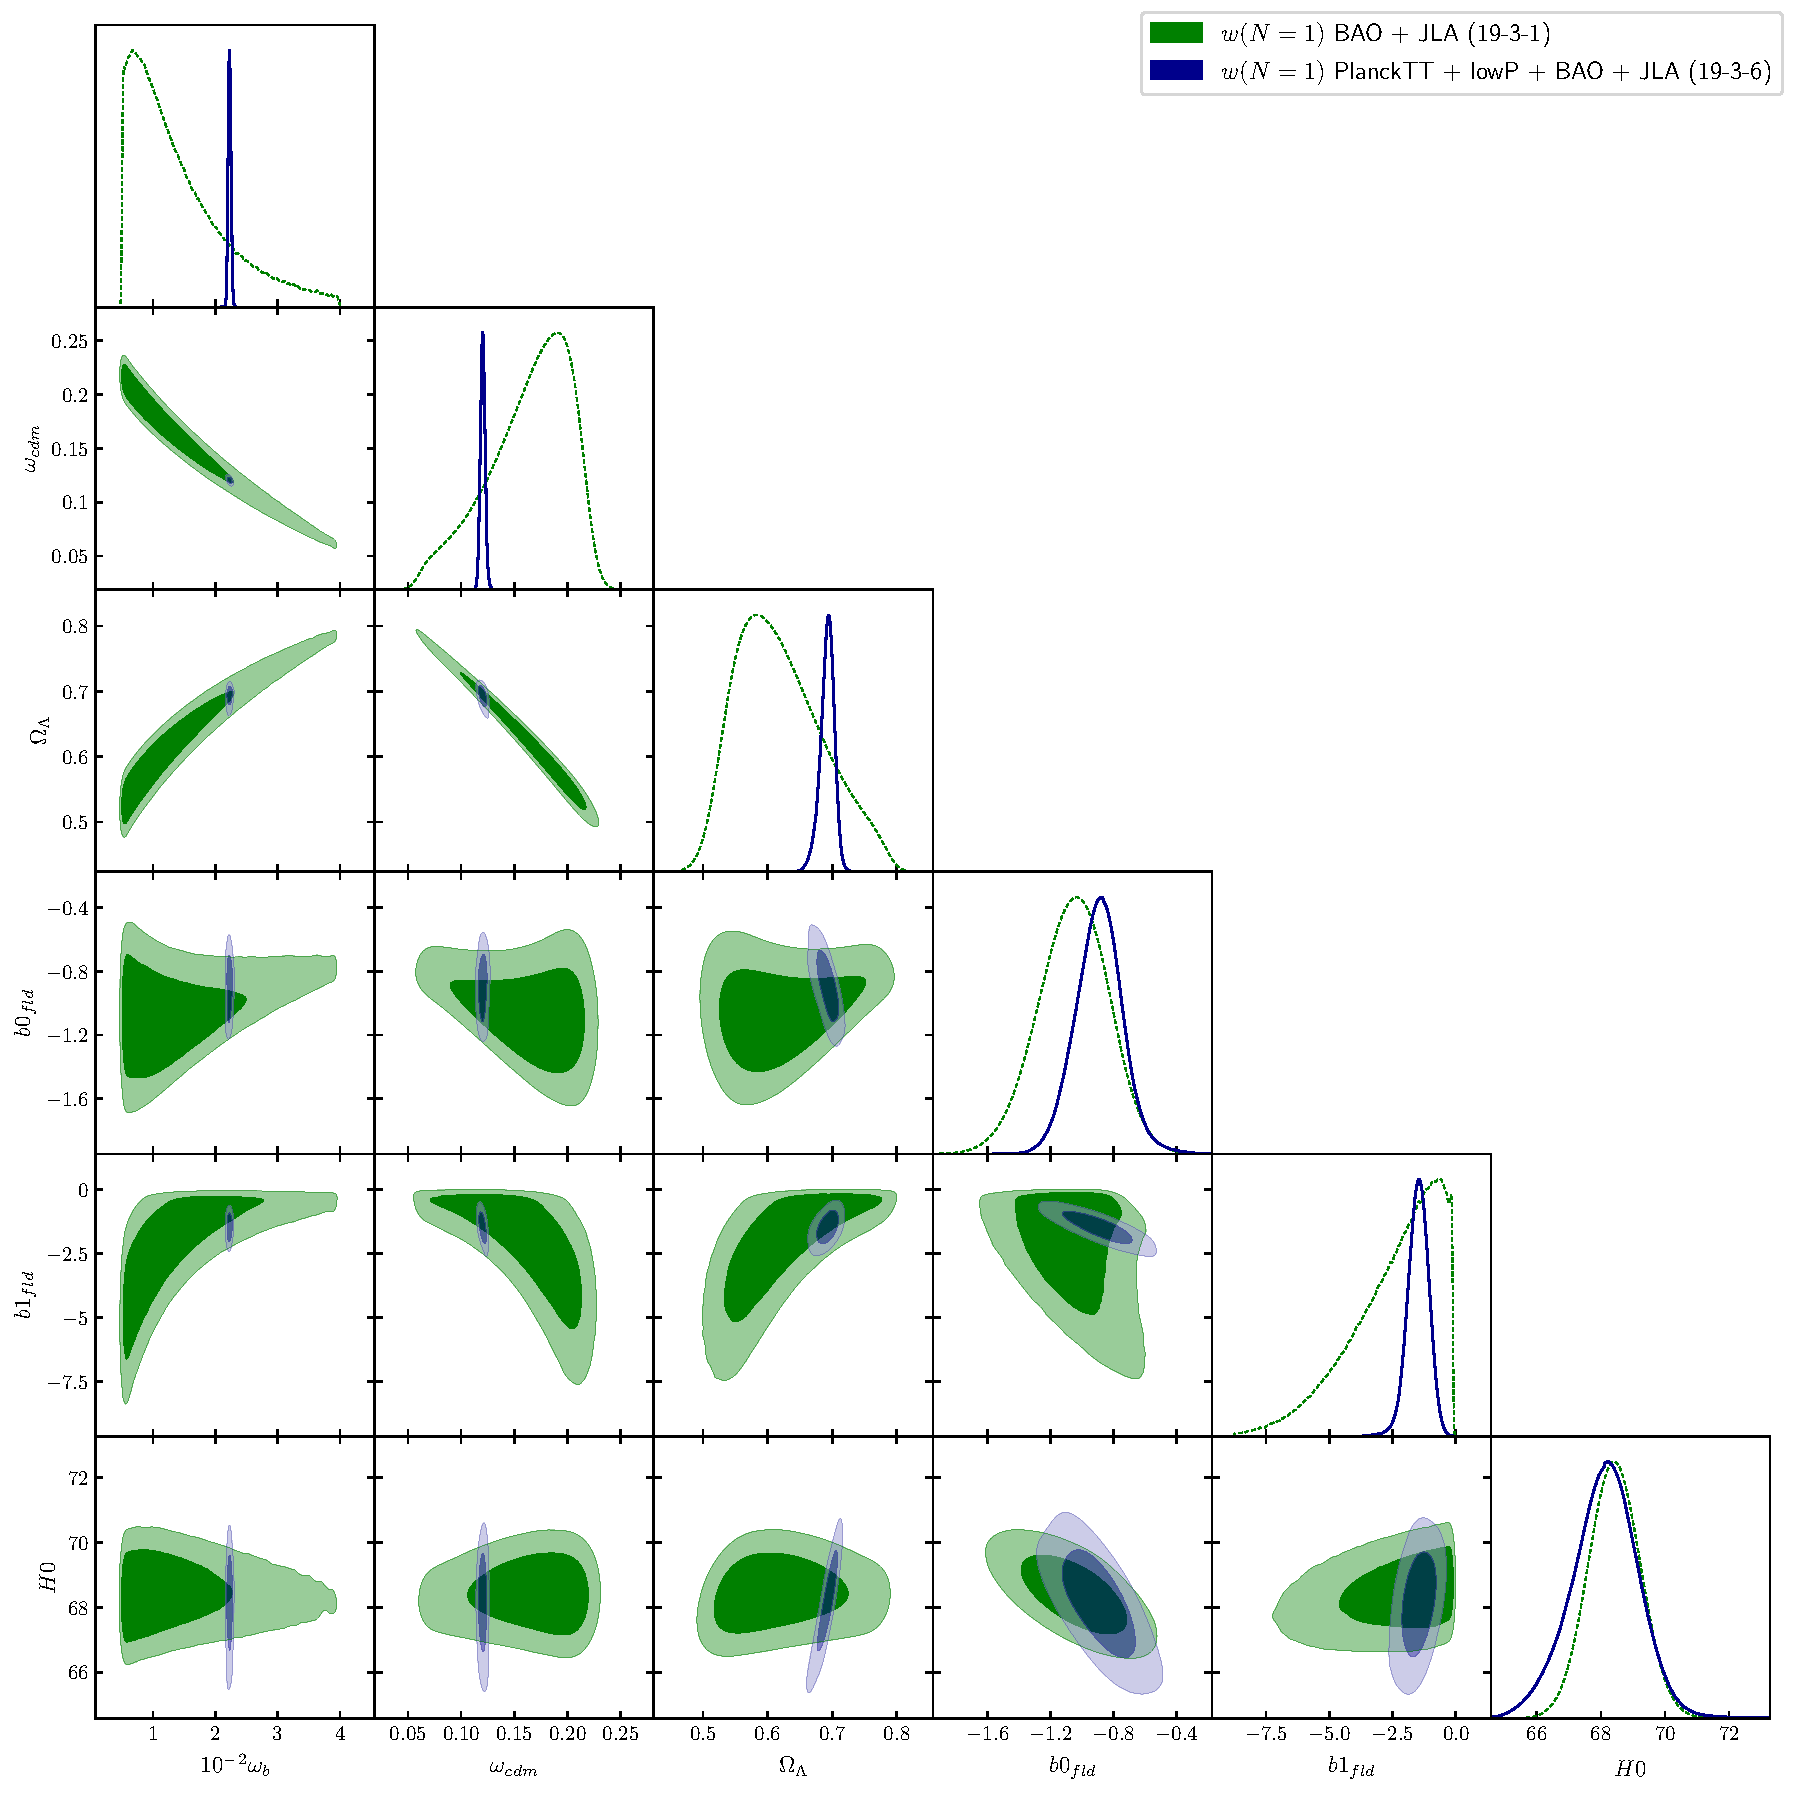
\includegraphics[scale=0.6]{N1_experiments_march.pdf}
 %\caption{\footnotesize{[mean, min, max, 1-sigma, scale, 'role']}}
\end{figure}

\subsection{w(N=2)}

\begin{itemize}
 \item BAO+JLA, 1.2m de pasos, 8 procesos, convergencia de todos los parámetros
 \item Planck+BAO+JLA, 1m de pasos, 6 procesos, convergencia parcial
\end{itemize}

\begin{tabular}{|l|c|c|c|c|} 
 \hline 
Param & best-fit & mean$\pm\sigma$ & 95\% lower & 95\% upper \\ \hline 
$100~\omega_{b }$ &$3.946$ & $1.675_{-1.2}^{+0.31}$ & $0.5$ & $3.528$ \\ 
$\omega_{cdm }$ &$0.06009$ & $0.1528_{-0.031}^{+0.058}$ & $0.06814$ & $0.2216$ \\ 
$b0_{fld }$ &$-1.136$ & $-1.209_{-0.28}^{+0.28}$ & $-1.785$ & $-0.633$ \\ 
$b1_{fld }$ &$1.845$ & $-1.404_{-2.5}^{+3.5}$ & $-7.434$ & $4.162$ \\ 
$b2_{fld }$ &$-4.629$ & $-4.69_{-3.9}^{+1.9}$ & $-8.793$ & $-0.3901$ \\ 
$\Omega_{\Lambda }$ &$0.79$ & $0.6403_{-0.097}^{+0.063}$ & $0.5151$ & $0.7834$ \\ 
$H0$ &$68.85$ & $68.71_{-0.91}^{+0.91}$ & $66.88$ & $70.53$ \\ 
\hline 
 \end{tabular} \\ 
$-\ln{\cal L}_\mathrm{min} =342.752$, minimum $\chi^2=685.5$ \\ 


\begin{tabular}{|l|c|c|c|c|} 
 \hline 
Param & best-fit & mean$\pm\sigma$ & 95\% lower & 95\% upper \\ \hline 
$100~\omega_{b }$ &$2.248$ & $2.24_{-0.018}^{+0.018}$ & $2.204$ & $2.275$ \\ 
$\omega_{cdm }$ &$0.1189$ & $0.1191_{-0.0017}^{+0.0019}$ & $0.1155$ & $0.1226$ \\ 
$10^{+9}A_{s }$ &$2.249$ & $2.238_{-0.08}^{+0.072}$ & $2.088$ & $2.395$ \\ 
$n_{s }$ &$0.9707$ & $0.9702_{-0.0048}^{+0.0044}$ & $0.9612$ & $0.9792$ \\ 
$\tau_{reio }$ &$0.08929$ & $0.08632_{-0.018}^{+0.018}$ & $0.0506$ & $0.1226$ \\ 
$b0_{fld }$ &$-1.118$ & $-1.053_{-0.19}^{+0.16}$ & $-1.399$ & $-0.7057$ \\ 
$b1_{fld }$ &$-0.5685$ & $-1.226_{nan}^{+nan}$ & $nan$ & $nan$ \\ 
$b2_{fld }$ &$-2.65$ & $-2.05_{nan}^{+nan}$ & $nan$ & $nan$ \\ 
$\Omega_{\Lambda }$ &$0.7002$ & $0.6987_{-0.0079}^{+0.0083}$ & $0.6825$ & $0.7146$ \\ 
$z_{reio }$ &$10.88$ & $10.6_{-1.5}^{+1.6}$ & $7.417$ & $13.71$ \\ 
$H0$ &$68.66$ & $68.54_{-0.83}^{+0.8}$ & $66.95$ & $70.12$ \\ 
$\sigma8$ &$0.8548$ & $0.853_{-0.019}^{+0.018}$ & $0.817$ & $0.8896$ \\ 
\hline 
 \end{tabular} \\ 
$-\ln{\cal L}_\mathrm{min} =5987.24$, minimum $\chi^2=1.197e+04$ \\ 




\begin{figure}[h]
 \centering
 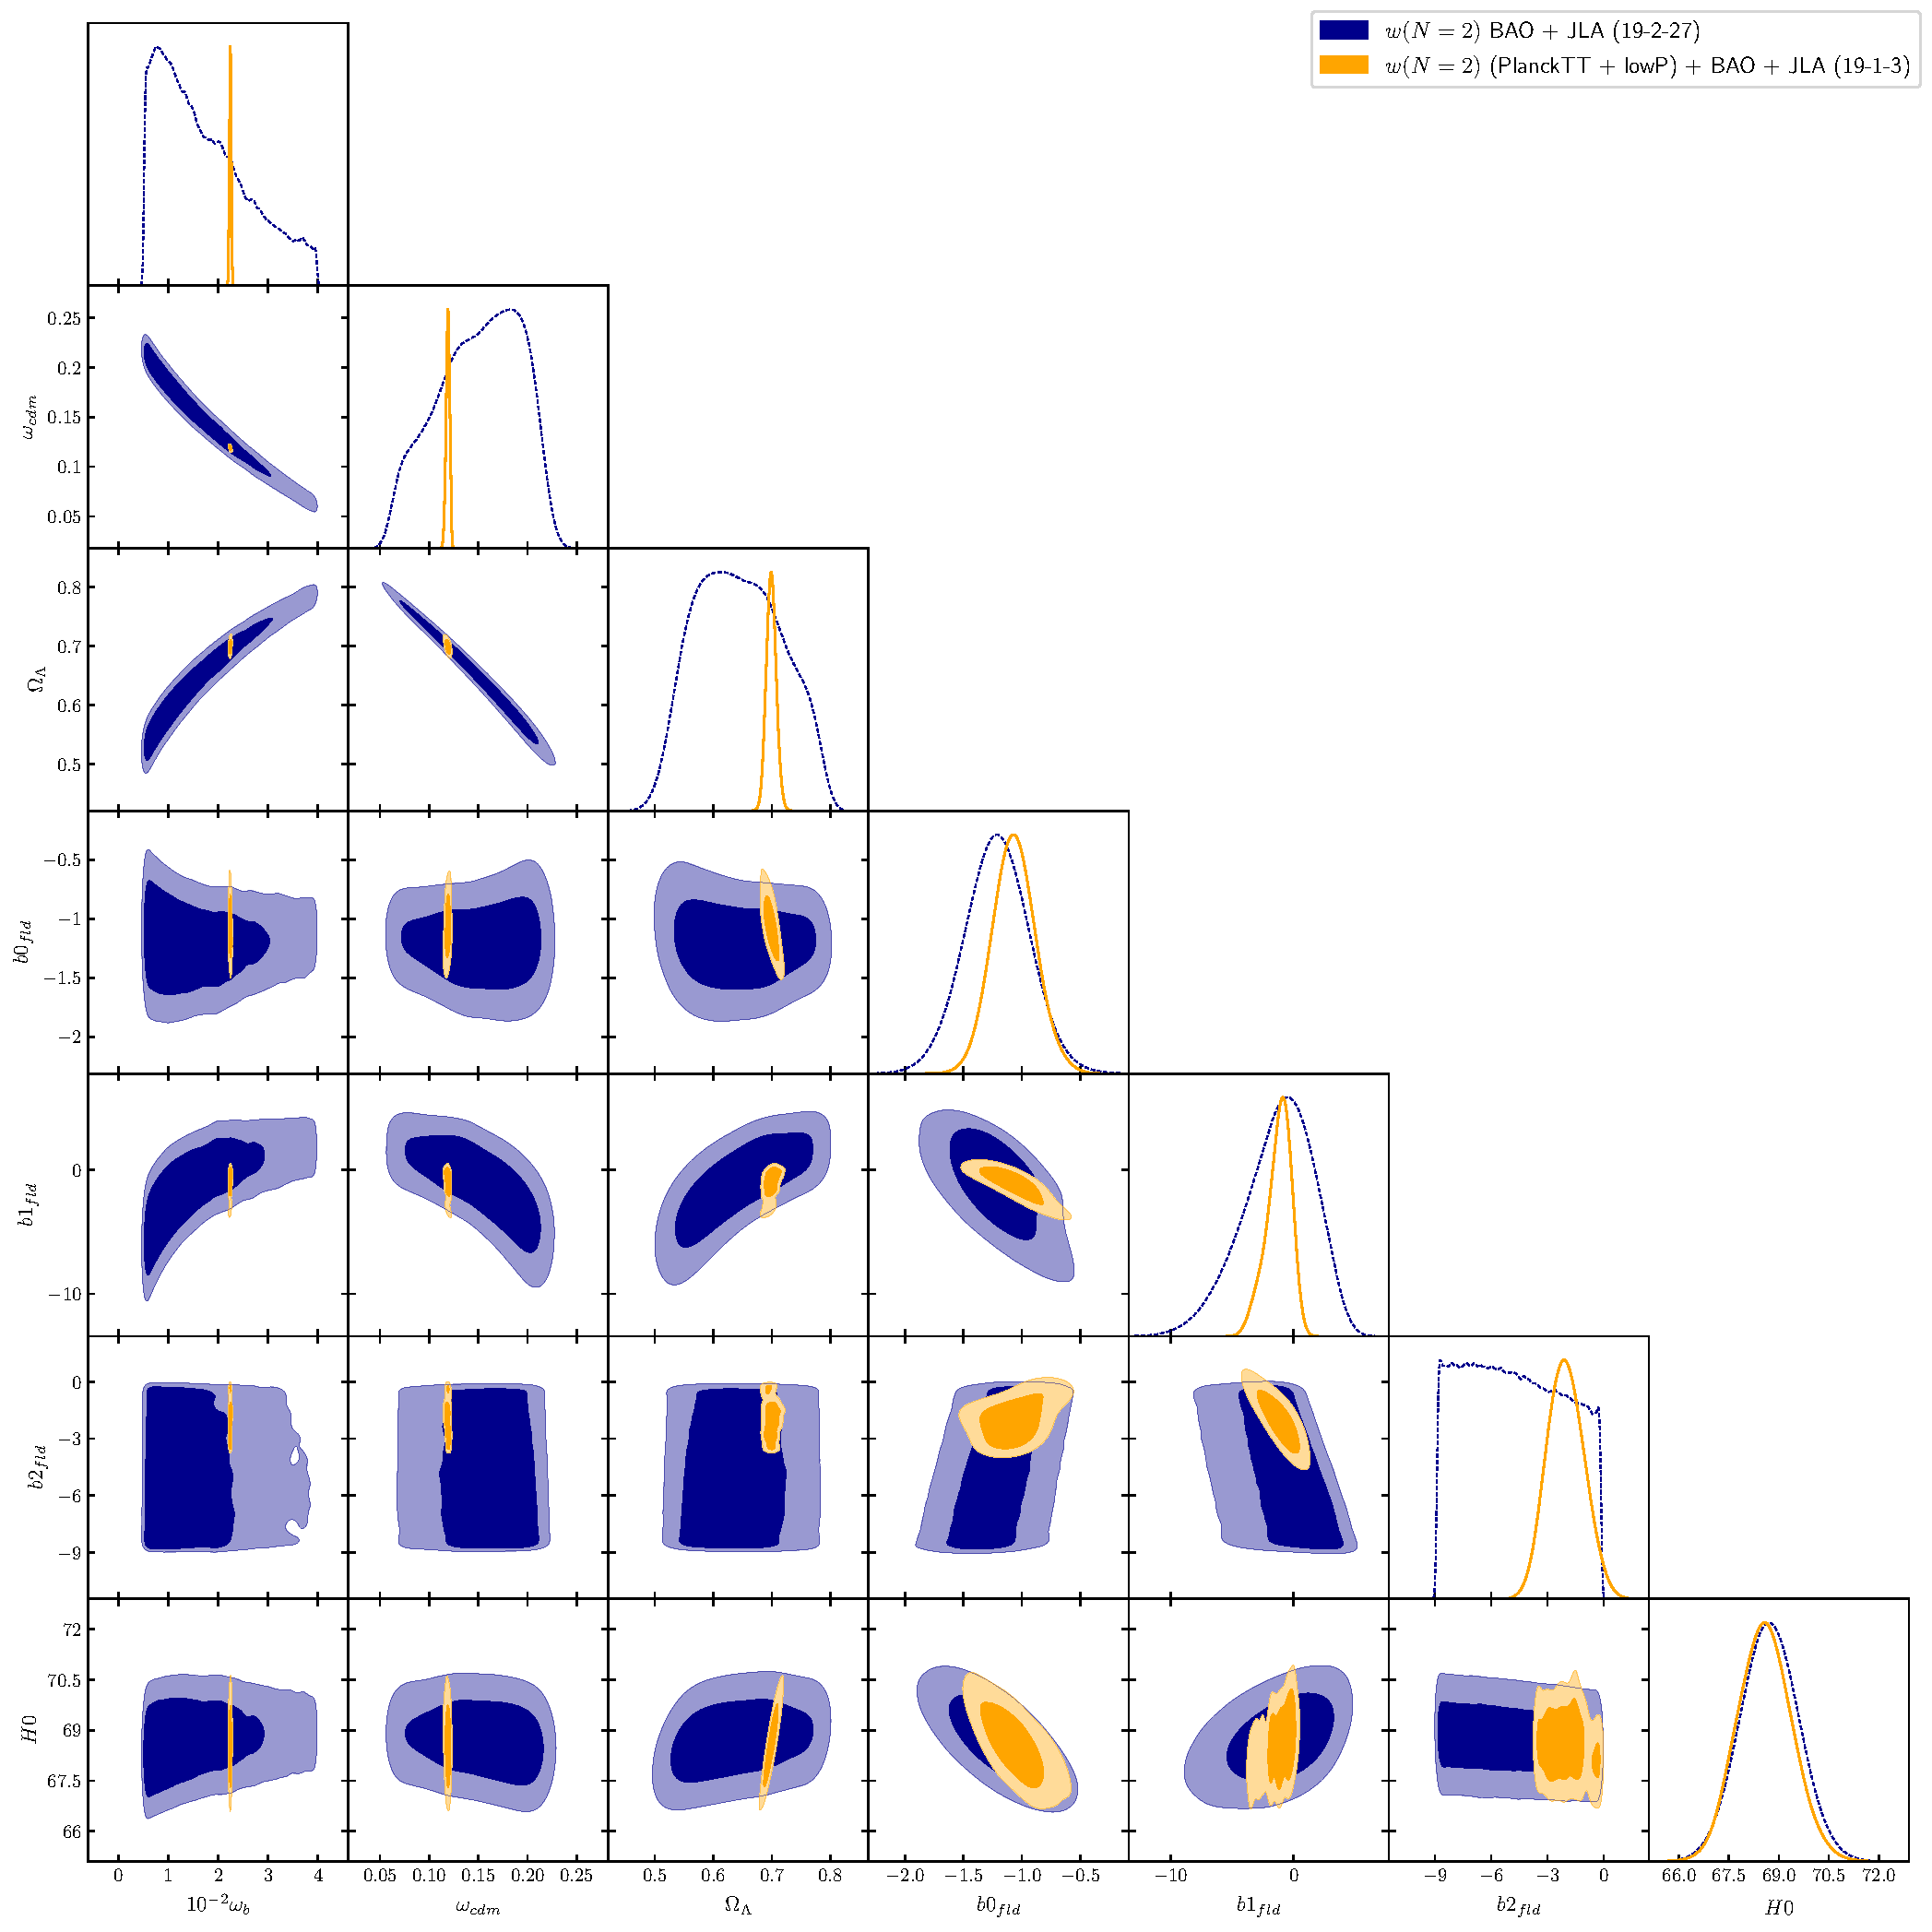
\includegraphics[scale=0.5]{N2_experiments.pdf}
 %\caption{\footnotesize{[mean, min, max, 1-sigma, scale, 'role']}}
\end{figure}

\begin{figure}[h]
 \centering
 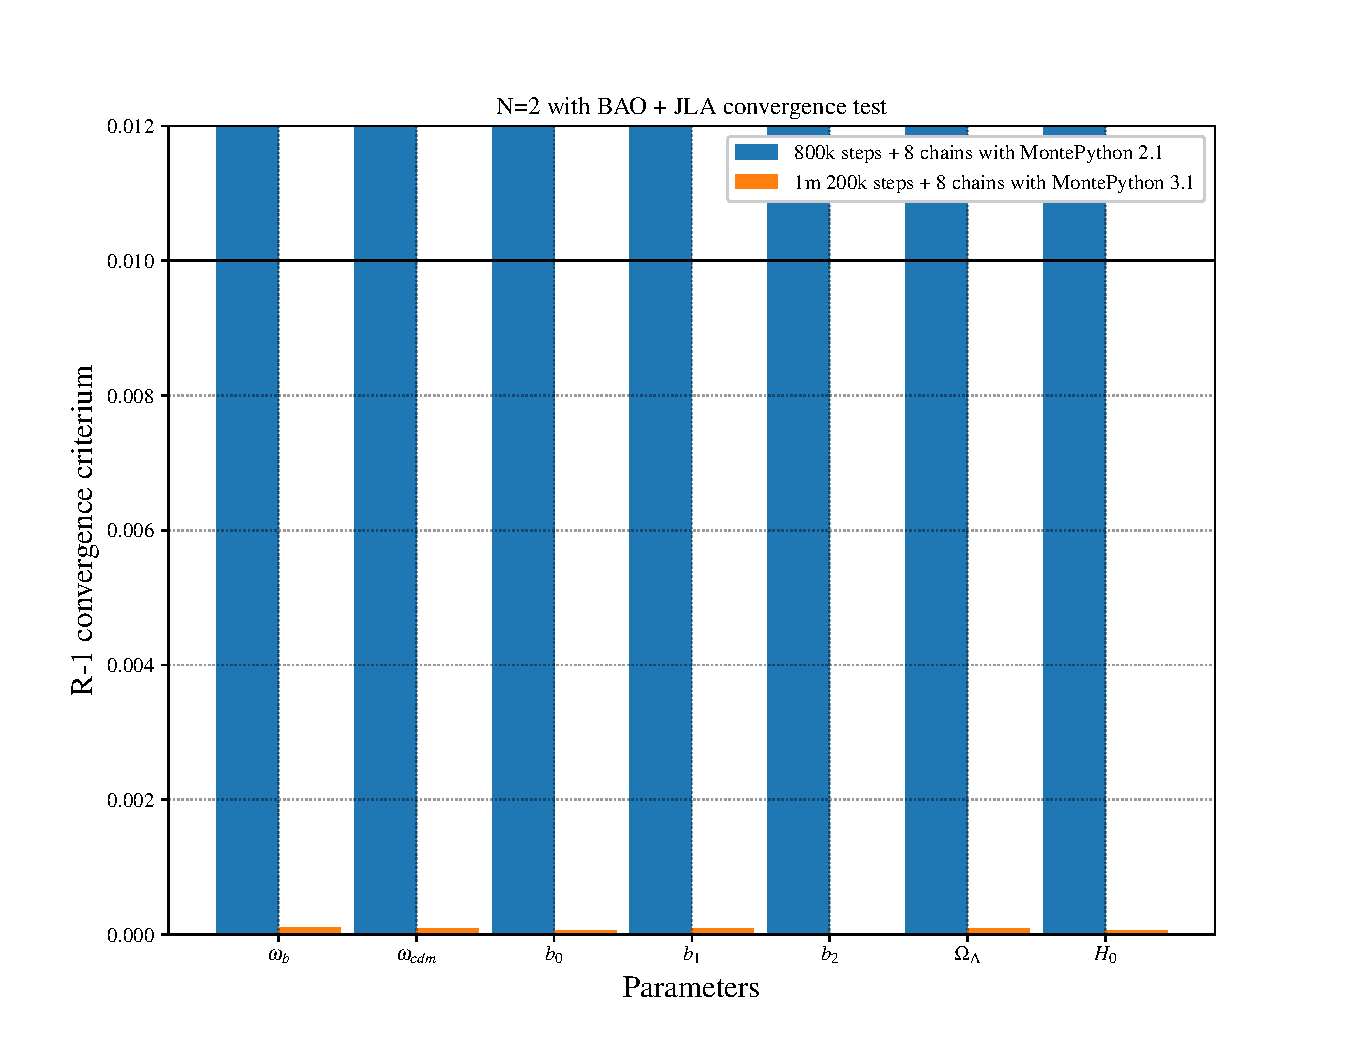
\includegraphics[scale=0.8]{plot_convergence_baojla_N=2.pdf}
 %\caption{\footnotesize{[mean, min, max, 1-sigma, scale, 'role']}}
\end{figure}

\end{document}